\documentclass{article}
\usepackage[utf8]{inputenc}
\usepackage{geometry}
\geometry{left=10mm, right=10mm, top=10mm, bottom=15mm}
%\usepackage{fullpage}
\usepackage{graphicx}
\usepackage{float}
\usepackage{blindtext}
\graphicspath{ {./bilder/} }
\renewcommand{\baselinestretch}{2}
\author{Jan Odermatt}
\title{Zusammenfassung Machinelearning}
\begin{document}
\tableofcontents
\section{Machine Learning Grundlagen}
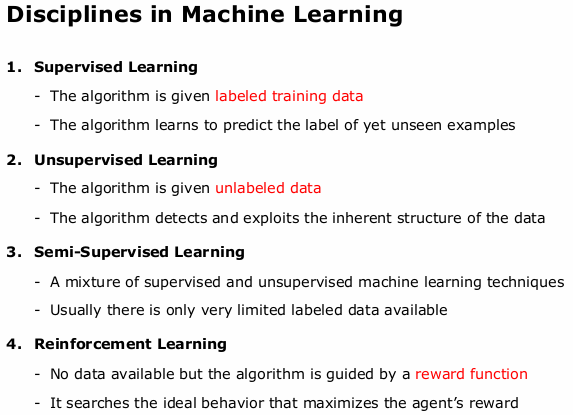
\includegraphics[width=0.4\textwidth]{disciplines_in_machine_learning.png}
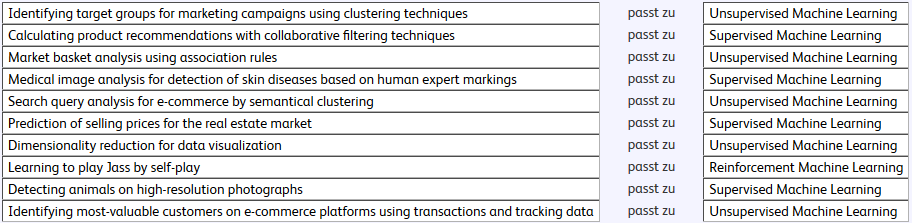
\includegraphics[width=0.6\textwidth]{disciplines_matched.png}
\section{Data Quality Assessment}
	\begin{enumerate}
		\item Data Cleaning\footnote{Auch wenn die Datenqualität selbständig verbessert werden kann sollten: alle Änderungen dokumentiert werden, data-repository mit versionierung verwendet werden, den Herausgeber der Daten auf fehler in den Daten hinweisen}
		\begin{enumerate}
			\item Dublizierte Daten erkennen und entfernen
			\item Daten mit nullen können ersetzt werden.
			\item Daten Machine Learning freundlicher gestalten (z.B. für Farben eigene Zeilen erstellen, damit die Euklid-Distanz gerechnet werden kann.
		\end{enumerate}
		\item Analyse mit Hilfe von
		\begin{enumerate}
		\item 5 Nummer Zusammenfassung (median Q2, Quartile Q1 und Q3 sowie min und max)
		\item Boxplots um das Datenset auf Ausreisser zu prüfen.
		\item Varianz und Standardabweichung berechnen
		\end{enumerate}
	\end{enumerate}
\section{Machine Learning Fundamentals}
	\begin{tabular}{c c c}
	  Euklid Distanz & Kosinus Ähnlichkeit & Formel\\
    	  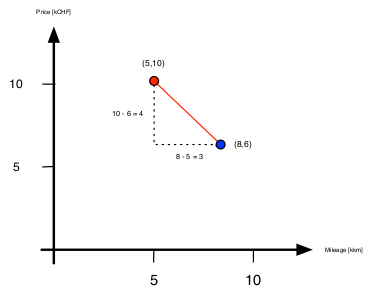
\includegraphics[width=0.25\linewidth]{euclide_distance.png} & 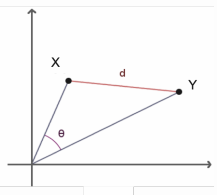
\includegraphics[width=0.25\linewidth]{cosine_similarity.png} & 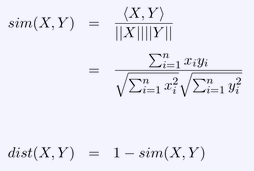
\includegraphics[width=0.25\linewidth]{cosine_similarity_formula.png} \\
	\end{tabular}
\section{Supervised Learning Basics}
\begin{figure}[H]
	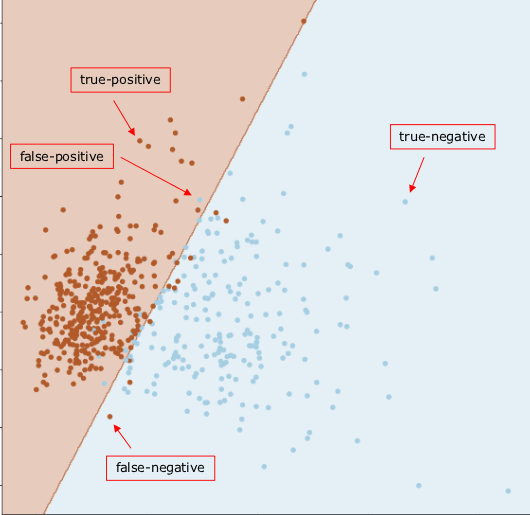
\includegraphics[width=0.5\linewidth]{true_positive}
\end{figure}
\begin{tabular}{c c}
	$Accuracy = \frac{TP + TN}{Total}$ & 	$Errorrate = \frac{FP + FN}{Total}$ \\
	$Sensitivity = \frac{TP}{Actual Yes}$ = $\frac{TP}{TP + FN}$ & $Specificity = \frac{TN}{ActualNo} = \frac{TN}{TN + FP}$ \\
	$Precision = \frac{TP}{Predicted Yes} = \frac{TP}{TP + FP}$
\end{tabular}
\section{Linear Regression}
	Das Modell hat generell die folgende Form:
	$$y = h_\theta(x) = \theta_0 + \theta_1 * x$$

	Korrelation liegt immer zwischen $-1 <= r <= 1$.
	$r = 0$ bedeutet, dass keine Korrelation herrscht und umso weiter $r$ von $0$ abweicht, 
	desto höher die Korrelation.
\end{document}
